\documentclass[tikz,border=8pt]{standalone}
\usepackage[T1]{fontenc}
\usetikzlibrary{calc}
\begin{document}
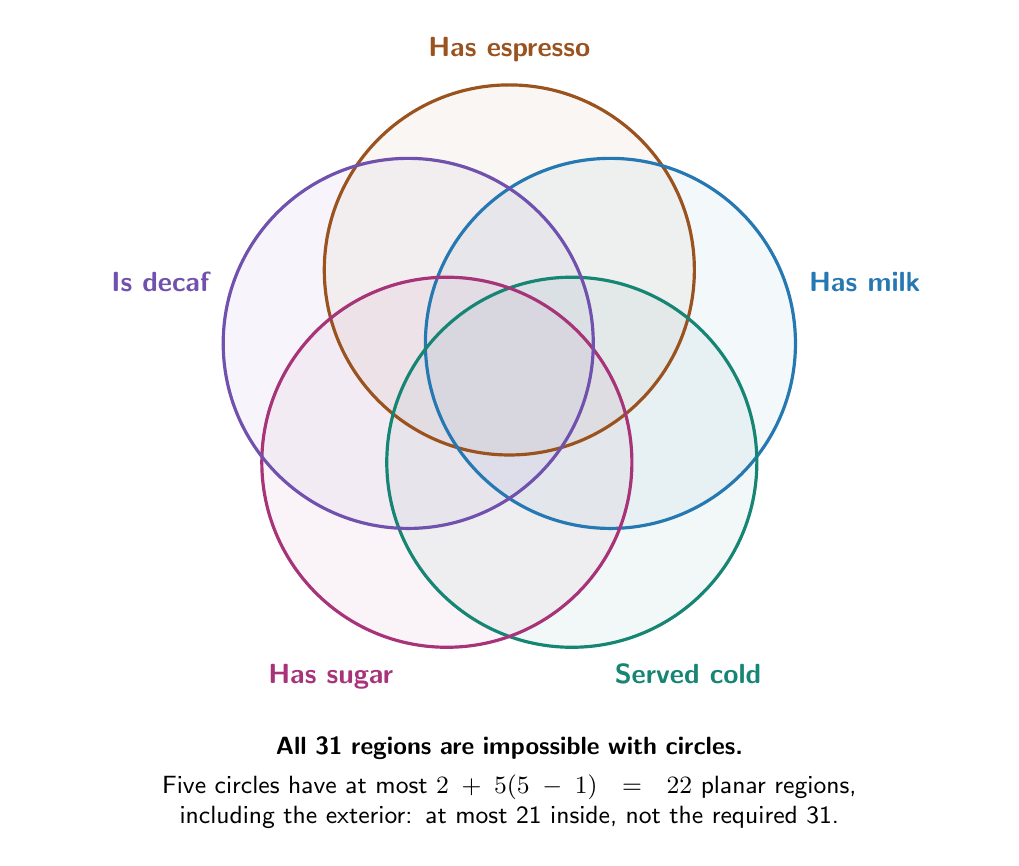
\begin{tikzpicture}[font=\sffamily, line width=1.15pt]
  \definecolor{espresso}{HTML}{9A531F}
  \definecolor{milk}{HTML}{2678B2}
  \definecolor{cold}{HTML}{168574}
  \definecolor{sugar}{HTML}{A73378}
  \definecolor{decaf}{HTML}{7051AE}

  % All ten pairs intersect twice; no three circumferences meet.
  % Thus this arrangement attains the maximum for five circles:
  % 22 planar faces, of which 21 lie inside the union.
  \coordinate (E) at (90:1.35);
  \coordinate (M) at (18:1.35);
  \coordinate (C) at (-54:1.35);
  \coordinate (S) at (-126:1.35);
  \coordinate (D) at (162:1.35);

  \foreach \center/\colour in {E/espresso,M/milk,C/cold,S/sugar,D/decaf}
    \fill[\colour,opacity=.055] (\center) circle[radius=2.35cm];
  \foreach \center/\colour in {E/espresso,M/milk,C/cold,S/sugar,D/decaf}
    \draw[\colour] (\center) circle[radius=2.35cm];

  \node[text=espresso,font=\sffamily\bfseries,above] at (90:3.86) {Has espresso};
  \node[text=milk,font=\sffamily\bfseries,right] at (18:3.86) {Has milk};
  \node[text=cold,font=\sffamily\bfseries,below,yshift=-0.4cm] at (-54:3.86) {Served cold};
  \node[text=sugar,font=\sffamily\bfseries,below,yshift=-0.4cm] at (-126:3.86) {Has sugar};
  \node[text=decaf,font=\sffamily\bfseries,left] at (162:3.86) {Is decaf};

  \node[align=center,text width=12cm,anchor=north,font=\sffamily\small]
    at (0,-4.45) {\textbf{All 31 regions are impossible with circles.}\\[3pt]
    Five circles have at most $2+5(5-1)=22$ planar regions,\\
    including the exterior: at most 21 inside, not the required 31.};
\end{tikzpicture}
\end{document}
